\section{Introduction}
In this chapter, we present our concepts in which R-Pulsar have been build upon.

\section{Framework}

R-Pulsar is a software stack that extends cloud capabilities to edge devices, allowing to collect and analyze data closer to the source of information and react autonomously to local events.

R-Pulsar uses a distributed architecture by the means of an overlay network, where each node in the overlay network is called a Rendezvous Point (RP). RPs can be a gateway located at the edge of the network or a server located in the cloud. R-Pulsar targets applications that span the cloud and the edge of the network.

R-Pulsar consists of five layers: (1) the location-aware self-organizing overlay, (2) the content-based routing layer, (3) the serverless messaging layer, (4) the memory-mapped data-processing layer, and (5) the programming abstraction layer.

\subsection{Location-aware Overlay Network Layer}

\begin{figure}[!h]
  \centering
  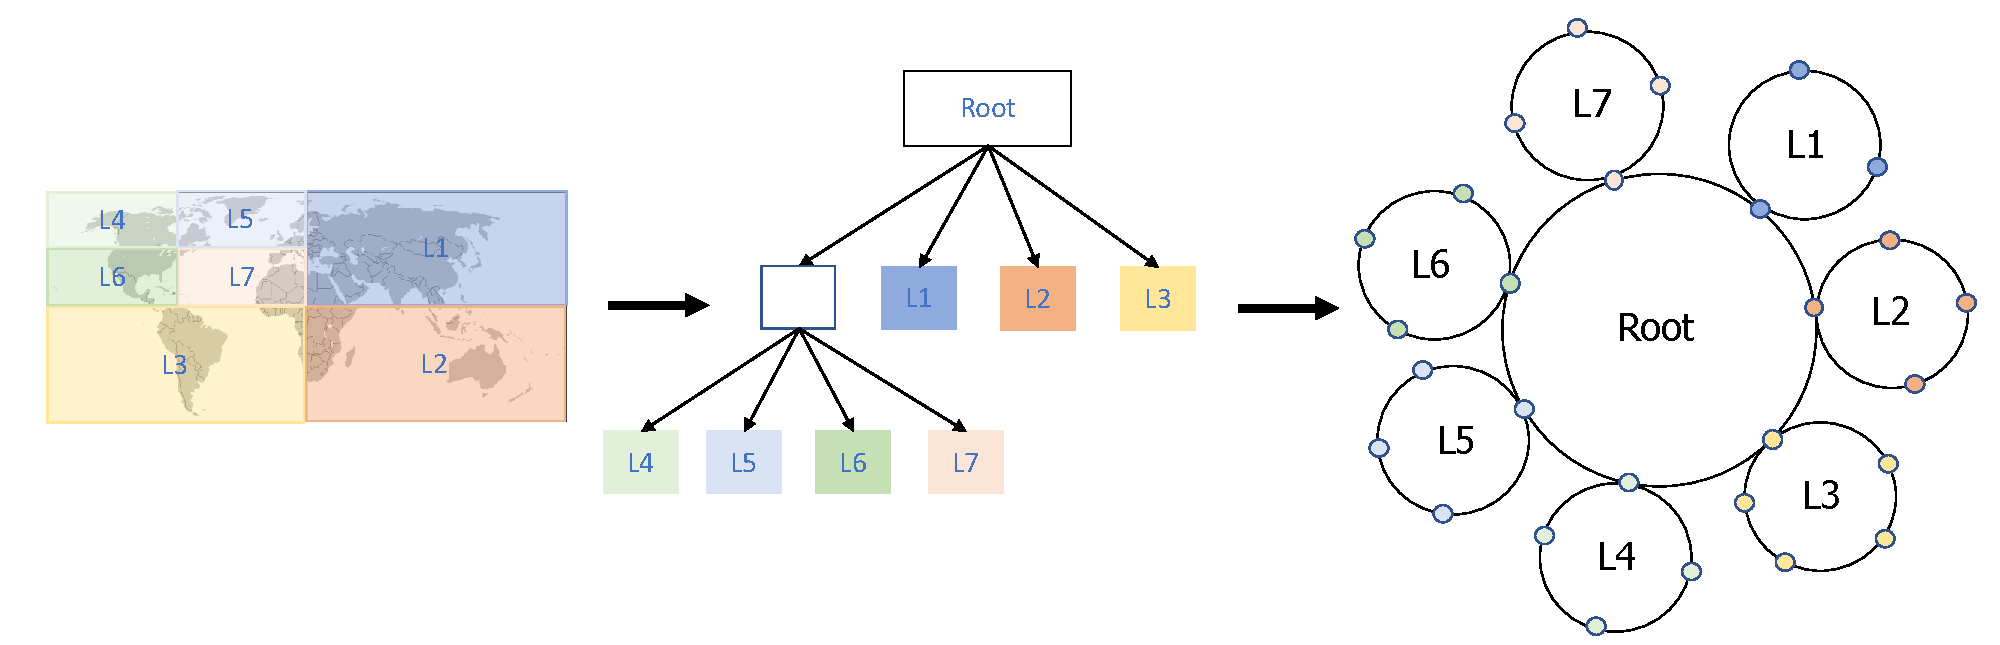
\includegraphics[width=1\columnwidth]{Figures/quadtree.pdf}
  \caption{}\label{fig:quadT}
\end{figure}

IoT data comes with temporal and spatial information, which is directly associated with their business value in a given context. Hence, IoT applications must process data in a timely fashion and from proper locations. In order to process data from the right location R-Pulsar uses a location-aware overlay network in conjunction with a point quadtree to logically groups of RPs that are physically close together. A point quadtree is a tree data structure in which each internal node has exactly four children. Each node represents a 2D bounded box covering a specific part of the space to index, using a root node to cover the entire area.

%The RPs are grouped based on the geographical location to guarantee that data gets processed with minimal latencies.

The R-Pulsar overlay network is an n-dimensional self-organizing structured overlay composed of RP nodes. Peers in the overlay can join or leave the network at any time. Every node in the overlay is assigned a unique identifier that consists of a 160bit unique identifier. Each node stores the keys that maps to the segment of the curve between itself and its predecessor node.

During the initialization of the overlay network, the RP attempts to discover an already existing RP in the system and construct its routing table. The joining RP sends a discovery message to the group. If the message remains unanswered after a duration (in the order of seconds), the RP assumes that it is the first in the system and it becomes the master RP, creating a single overlay network (Peer-to-Peer network). Every time any other RP joins the overlay network and the master RP responds to the discovery message, the  RP is added to the system by using the location of the RP and determining which quadrant the RP occupies. Once the initial P2P network has a sufficient number of RPs to guarantee that in case of multiple failures the P2P network will not disappear, the quadtree subdivides the overlay network into four additional P2P rings, plus an extra ring that will allow all the master RPs of each ring to communicate. Each RP master keeps a copy of the quadtree, so in the case of an RP failure the overlay network structure will never be lost. In the case of a master RPs failure, a master RP election is performed using the Hirschberg and Sinclair algorithm~\cite{Hirschberg}. Figure~\ref{fig:quadT} is a graphical representation of the quadtree and the logical organization of the P2P network.

In order to route a message the first strep is perform a quadtree query to decide in which of the P2P rings needs to be routed to. The locations in the AR message is used to perform a lookup in the tree and find the P2P ring closes to the given location. 

\subsection{Content-based Routing Layer}\label{sec:frameworkc}

\begin{figure}
\centering
\begin{subfigure}[b]{0.9\textwidth}
   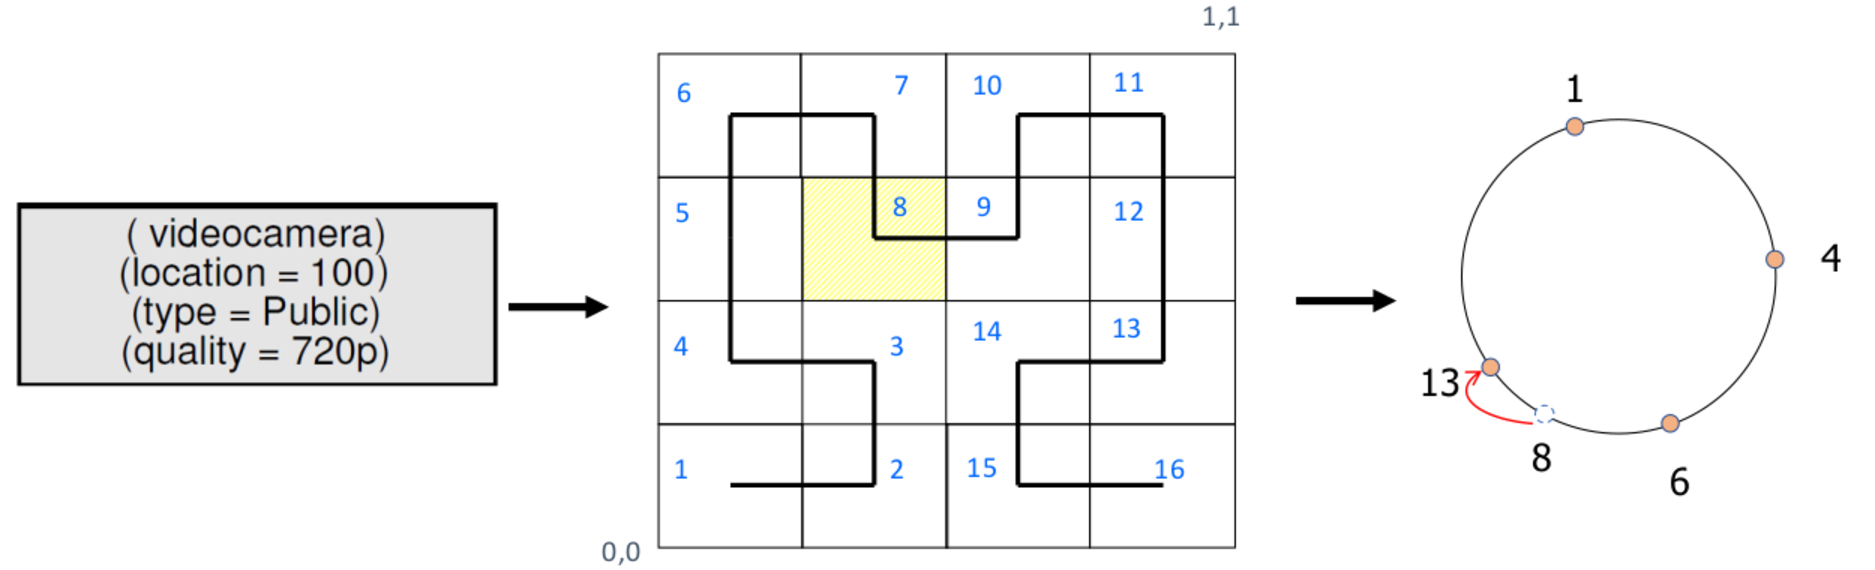
\includegraphics[width=1\linewidth]{Figures/single.pdf}
   \caption{}
\end{subfigure}
\begin{subfigure}[b]{0.9\textwidth}
   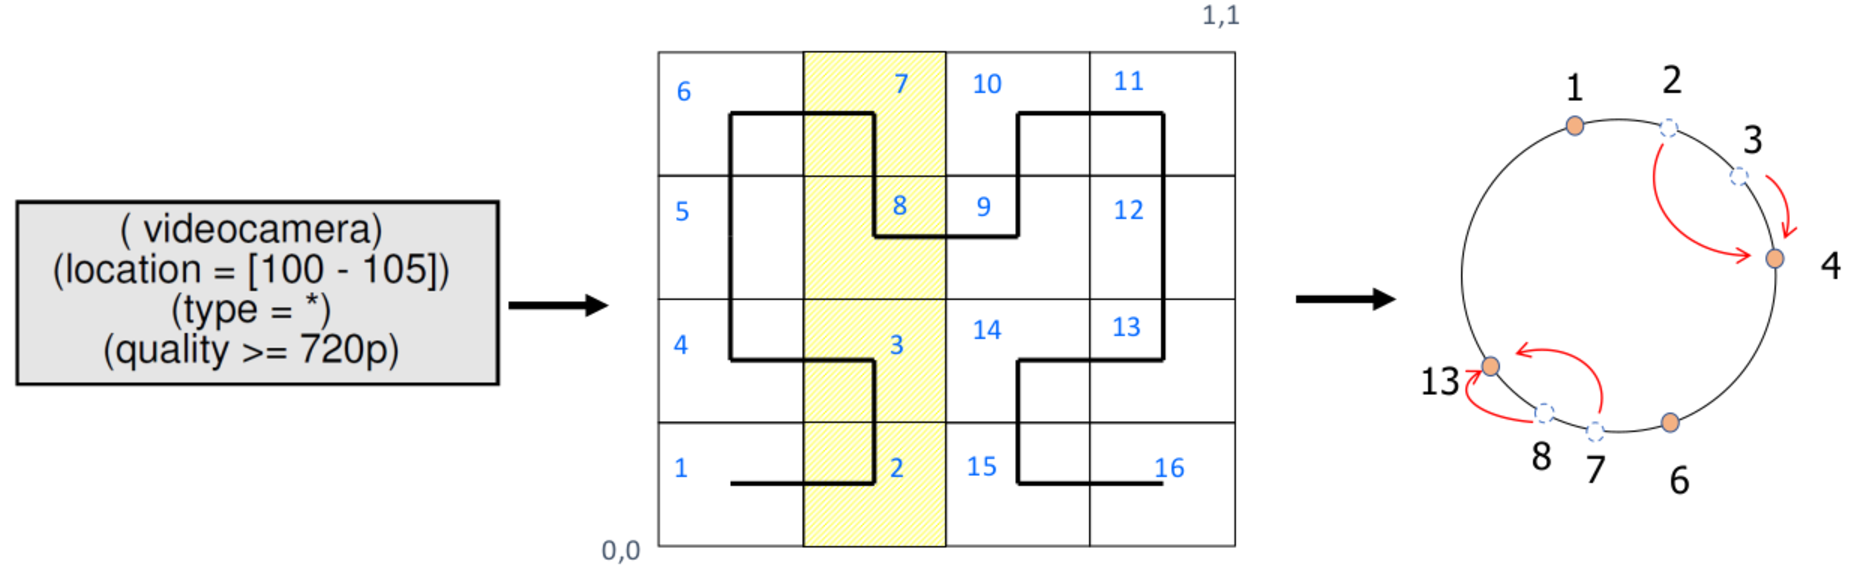
\includegraphics[width=1\linewidth]{Figures/multi.pdf}
   \caption{}
\end{subfigure}
\caption{R-Pulsar space filling curve routing using simple (a) and complex (b) profiles.}\label{fig:routingProfiles} 
\end{figure}

%As mentioned above, the lookup operator provided by the location-aware overlay requires an exact identifier, the AR message and the location to be routed.

This layer builds on top of the location-aware overlay to route messages. The content-based routing layer maps AR profiles onto single identifiers or clusters of identifiers to enable information discovery using partial knowledge, as described in \cite{SCHMIDT2008962}.

Content-based routing is achieved by performing two steps: The first step is to encode the set of attributes and/or attribute-value pairs of the AR message, into a set of unique base 10 ids. The second step is to use the set of base 10 numbers produced in the previous step and pass them to the Hilbert Space Filling Curve (SFC). The SFC~\cite{SFC} is used to map the n-dimensional space of the AR profile to the one-dimensional space ID of the location-aware overlay network. Content based routing can be performed in two ways using simple keyword profiles or complex keyword profiles, the routing process is described below.

\textbf{Routing using simple keyword profiles:} The routing process consists of two steps. At the first step, the AR profile containing only exact attribute-value pairs is encoded into a set of based 10 ID's, each id represents an exact attribute-value pair of the AR profile, then the set of base 10 ID's are passed to the SFC to obtain a single based 10 ID. This base 10 ID corresponds to 160bit unique identifier used by the P2P overlay network. Figure~\ref{fig:routingProfiles}a illustrates this process. \vspace{1ex} 

\textbf{Routing using complex keyword profiles:} Similarly to the first step, an AR profile this time contains wildcards, ranges, or both is encoded and a set of base 10 ID's. The wildcard gets replaced for each of the possible value in the alphabet, producing multiple base 10 encoding sets. This sets of encoding are passed to the SFC to obtain a single based 10 ID, this step is repeated for each of the base 10 encoding sets. Then we end up with muntiple base 10 IDs that corresponds to several 160bit unique identifiers of the P2P overlay network. Figure~\ref{fig:routingProfiles}b illustrates this process.

\subsection{Serverless Messaging Layer}\label{sec:serverless}

%\begin{figure}[!h]
%  \centering
%  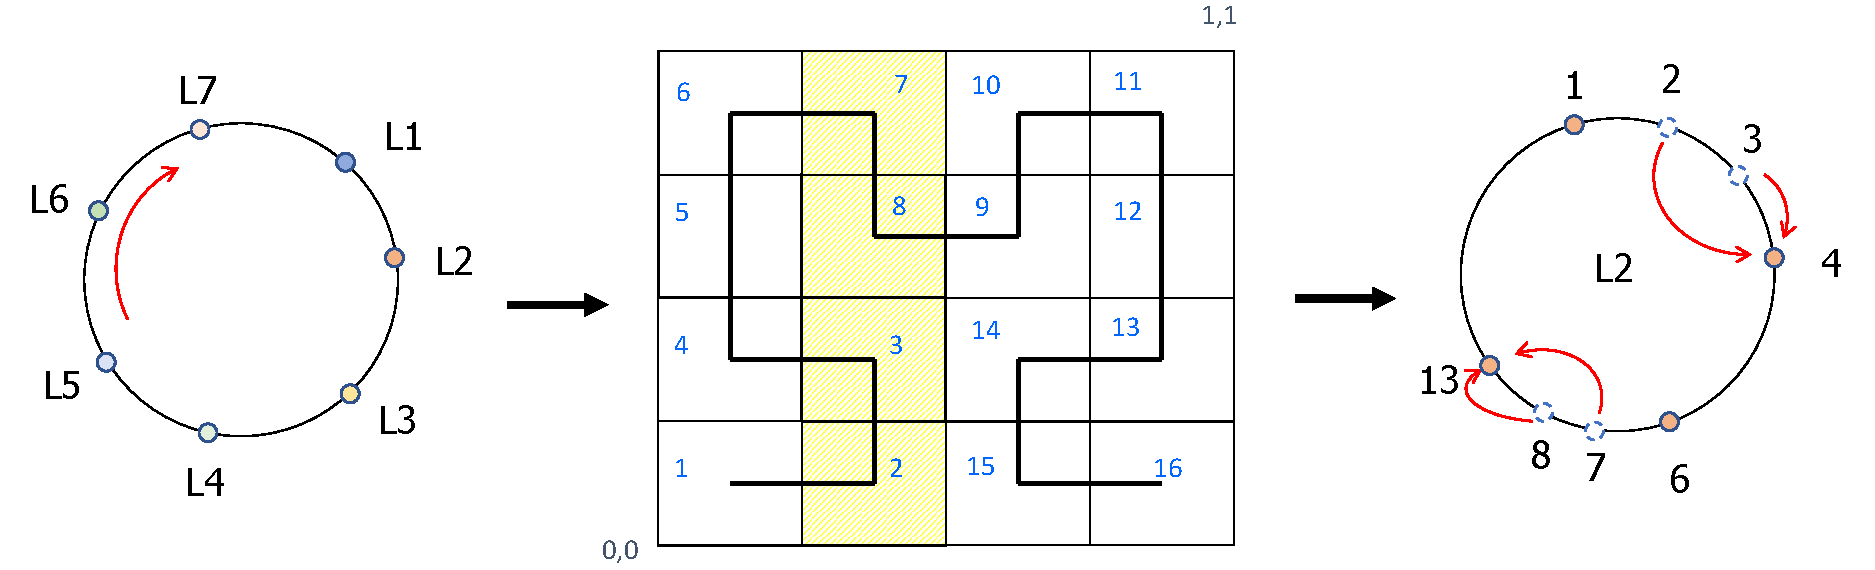
\includegraphics[width=0.9\columnwidth]{Figures/multi-old.pdf}
%  \caption{}\label{fig:Multiquad}
%\end{figure}

Serverless computing is a cloud computing model that aims to abstract server management and low-level infrastructure decisions away from developers. Allowing to deploy and execute pieces of code in response to events without the need to specify IP addresses. The serverless messaging layer implements the AR interaction model described in Chapter~\ref{chap:AR} and it consists of two components: the matching engine and the profile manager. 

The matching engine component is essentially responsible for matching profiles. If the result of the match is positive, then the action field of the incoming message is executed first, followed by the evaluation of the action field in the matched profiles. 

The profile manager manages locally stored profiles and monitors message credentials and contexts to ensure that related constraints are satisfied.

\begin{table}[h]
\begin{tabular}{cc}
\hline
\textbf{Operators}                       & \textbf{Guarantees}                                                                                                                                                                                                    \\ \hline
bool \textbf{init()}                             & \begin{tabular}[c]{@{}c@{}}Connects to the existing P2P network \\ and guarantees the discover all existing RPs\end{tabular}                                                                                           \\ \hline
bool \textbf{post}(AR Message)                   & \begin{tabular}[c]{@{}c@{}}Routes the AR Message based on the \\  profile and the location;\\  Guarantees that all RPs responsible for that \\  content in that location will receive the \\  AR message.\end{tabular} \\ \hline
bool \textbf{stream}(AR Message, String Peer Id) & \begin{tabular}[c]{@{}c@{}}Stream direct messages to a select RP.\\ Guarantees that the responsible RP will\\ always receive the message.\end{tabular}                                                                 \\ \hline
AR Message \textbf{poll}()                       & \begin{tabular}[c]{@{}c@{}}Retrieve messages from a select RP point.\\ Guarantees that the consumer will always\\ receive the message.\end{tabular}                                                                    \\ \hline
\end{tabular}
\centering
\caption{Available R-Pulsar operators.} \label{tb:operators}
\end{table}

The serverless messaging layer offers four different operators. Table~\ref{tb:operators} summarized all of the available operators.

The \textbf{init}() operator is used to join the R-Pulsar network and it guarantees that all the available RPs will be discovered.

The \textbf{post}(AR message) operator is used to route the messages without the need of specifying the recipient of the message, the recipient of the message is resolved by using the AR Message. To route a message using the post abstraction the following steps are performed:

The \textbf{stream}(AR Message, String Peer Id) operator is used to stream data directly to a specific RP, this operator bypasses the location and the content based routing layers.

The \textbf{poll}() operator is used to retrieve the data other RPs are sending.

\begin{itemize}
    \item Step 1: The location specified in the AR message is used to the location aware layer which is responsible for performing a location query in the quadtree. The result of the query is the P2P network that will receive the message.
    \item Step 2: Once the P2P network is selected, then content of the AR profile is used to select which RP will be responsible for the message. The content based layer is responsible for encoding the AR profile into a set of base 10 ids and performing a SFC call to go from n-dimentional space to 1-dimensional space base 10 id.
    \item Step 3: The base 10 id is used to route the message to the right RP.
\end{itemize}

\subsection{Memory-mapped Streaming Analytics Pipeline}
The data pipeline is responsible for consolidating data from multiple sources, processing the data, and making them available to be used. State-of-the-art data pipelines are known to be data-intensive tasks, resulting in the inability to performing real-time data analytics when deployed on constrained devices. The memory-mapped streaming analytics pipeline layer is motivated to overcome that issue.

The streaming analytics pipeline comprises the following layers: 

\begin{enumerate}

\item The data collection layer gathers data from multiple sources and brings them to the pipeline.
\item The stream processing layer processes the data and performs computations on the collected data.   
\item The data storage and query layer reads and writes data to the main memory and disk.

\end{enumerate}

\subsubsection{Data Collection Layer}
\hfill\\
Multiple data collection services are available, such as Apache Kafka~\cite{kafka}, Google Pub/Sub~\cite{google}, Amazon Firehose~\cite{amazon}, and Mosquitto~\cite{mosquitto}. Although some are designed to be deployed on edge devices, these services offer limited performance when deployed in constrained devices due to the limited read and write disk speeds.

We designed and implemented a custom data collection layer designed specifically for constrained devices using a memory-mapped queue. A memory mapped file is a segment of virtual memory that has been assigned a direct correlation with some portion of a file. This file is physically present on disk, which allows the operating system to ensure data access operations with better performance than standard file access. The core principle of the R-Pulsar queue system emerges from the observation that random memory read is about 3.5x faster than sequential disk read, as measured in Table~\ref{tb:table1}. 

The trade-off of using a memory mapped data collection system is that operating systems decides when to copy data from the main memory to disk. %Our approach is based on the assumption that the MQTT protocol assumes that the client and the server are generally available~\cite{IBM-MQTT}. 

\begin{table}[h!]
\scalebox{1.2}{
\begin{tabular}{|l|c|c|}
\hline
\multicolumn{1}{|c|}{\textbf{Operation}} & \textbf{Disk} & \textbf{RAM Memory} \\ \hline
Sequential read                          & 18.89 MB/s             & 631.34 MB/s \\ \hline
Sequential write                         & 7.12 MB/s              & 573.65 MB/s \\ \hline
Random read                              & 0.78 MB/s              & 65.96 MB/s              \\ \hline
Random write                             & 0.15 MB/s              & 65.88 MB/s              \\ \hline
\end{tabular}}
\centering

\caption{Measurements of Disk I/O vs RAM memory performance on a Raspberry Pi.} \label{tb:table1}
\end{table}

\subsubsection{Data Processing Layer}
\hfill\\
R-Pulsar can be used on top of any data processing engine, allowing the end user to choose his or her favorite data-processing engine. The current release of R-Pulsar was validated using Apache Edgent. 

\subsubsection{Data Storage and Query Layer}
\hfill\\
This layer leverages the AR programming abstraction and a key-value database to offer SQL-like query capabilities. The storage layer uses the SFC of the content-based routing layer to allow the ability to perform wildcard, range, or exact queries and allows the data to be horizontally partitioned among multiple RPs. 

For storing data, R-Pulsar relies on RocksDB~\cite{rocks}, an embedded key-value database optimized for fast and low-latency storage. The database keeps the most recently used data in the main memory and stores the least recently used data on disk.

\subsection{Rule-based Programming Abstraction}\label{sec:programming-data}
The rule-based programming abstraction makes it possible to build IoT applications and decide \textbf{when} data must be sent to the cloud for further postprocessing without having to manage any infrastructure.

It consists of a rule engine that allows developers to specify IF-THEN rules that can trigger other data-processing tasks when a condition is satisfied. The THEN clause of the conditions sends an AR message with a custom profile to start and stop data-processing tasks on demand. %The design and evaluation of the rule-based programming abstraction were illustrated in our previous paper~\cite{rules}.

We created a rule-based system, which contains all of the appropriate knowledge encoded into a set of If-Then rules. The system examines all the rule conditions (IF) and determines a subset, the conflict set, of the rules whose conditions are satisfied based on the data tuples. Out of this conflict set, one of those rules is triggered (fired). When a rule is fired, the action specified in its THEN clause is carried out. The loop for firing rules continues until one of two conditions are met: there are no more rules whose conditions are satisfied or a rule is fired. We allow to specify two different types of rules, ones that let you express data quality requirements which impose time constraints on the processing of the tuples, allowing the specification of a trade-off between the data quality and computational complexity. And the second one that offers the ability to express content-driven rules which complement the data quality requirements by triggering further stream-processing topologies either at the core or at the edge of the network if the data needs further processing due to quality of the data.

\subsubsection{Content-Driven Rule-Based System}
The content-driven rules consists of a single rule table that contains a set of rule entries installed by the developer. The rule entries contain a collection of conditions, a single action, and a single priority field.

The priority field is used in the event of having two or more rules that satisfy the condition, in order to brake the tie, only the one with highest priority will be executed. The condition field consists of one ore multiple antecedents (If clause). The antecedent of a rule consists of two parts: an object and its value. The object and its value are linked by an operator. The operator identifies the object and assigns the value. The following are all the operators currently supported:
\textbf{AND}, \textbf{OR}, \textbf{NOT}, \textbf{$>$,$<$,$>=$,$<=$}, \textbf{==}, \textbf{AVG}, \textbf{MIN}, \textbf{MAX}, and \textbf{Standard Deviation}

The rule actions define what to do when the condition is satisfied, then the rule is fired and the action its performed. Each rule-entry has a single action associated with it; the three actions that are currently supported in our AR system are:

\begin{enumerate}
  \item \textbf{Store} the results of the computation at the Edge or the Cloud. This allows the topology developers to seamlessly store the results of the topology based on the content of the data across a federated set of resources and have the ability to locate where those data results have been stored when needed.
  \item \textbf{Trigger} a new Apache Storm topology, if it doesn't exist already, or route the tuples to an already running topology. Can be used to achieve multiple functionalities such as: split topologies/workflows across a set of participating Rendezvous Points that can be located at the core or at the edge of the network or make decisions based on the content of the data and triggering new computations.
  \item \textbf{Notify} action allows to notify any node part of the overlay network and stream the results to them.
\end{enumerate}


The following snippet of code shows how developers will express the content-driven rules to trigger a new topology in the cloud:

\begin{figure}[h!]
  \centering
  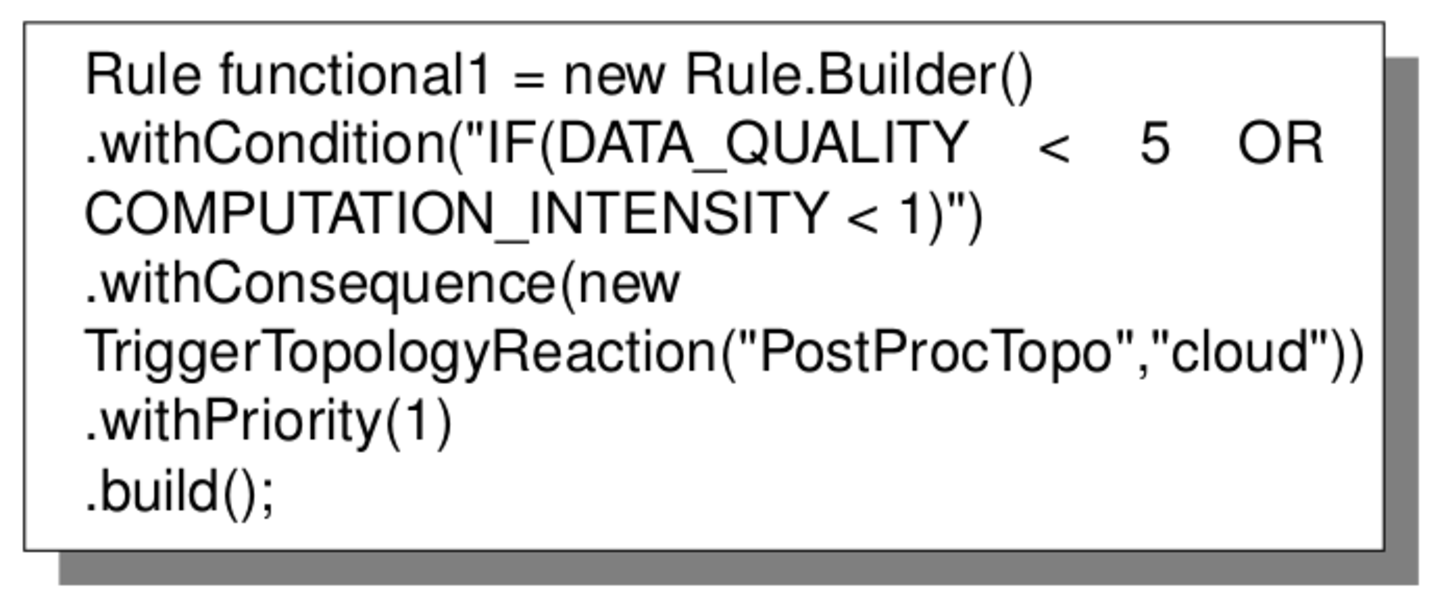
\includegraphics[width=0.7\textwidth]{Figures/RuleTopology.pdf}
  \caption{Trigger topology reaction rule definition.}
  \label{fig:RuleTopology}
\end{figure}


The 'withCondition' is the IF rule expression that has to be satisfied and the 'withConsequence' is the action that will be triggered when the rule is satisfied. The action has two parameters: the first one specifies the name of the topology that needs to triggered if it is the first time executing the action or route to that topology if its already running. The second parameter specifies where it needs to be triggered. In this case it will be triggered on the cloud nodes that are part of the overlay network since its really computationally intensive. 

Another brief code example of how developers will express the content-driven rules to store the matching results at the edge of the network:

\begin{figure}[h!]
  \centering
  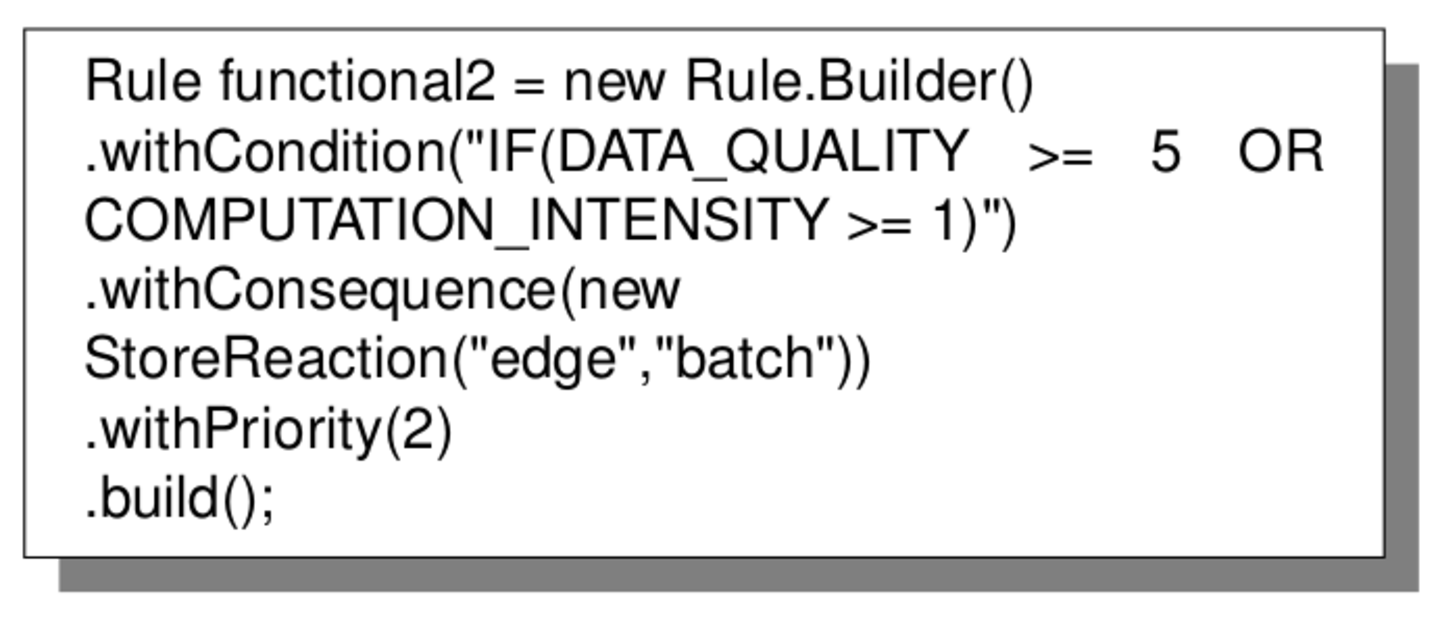
\includegraphics[width=0.7\textwidth]{Figures/StoreReaction.pdf}
  \caption{Store reaction rule definition.}
  \label{fig:StoreReaction}
\end{figure}


The action of this second rule also has two parameters: the first parameter specifies where to store the results of the streaming computation, which in this case, is at one of the edge nodes that are part of the overlay network since we want to be able to get our results quickly. The second parameter specifies how to store the results either one by one (streaming fashion) or batch (several at a time).

Rules programming abstraction can be used to evaluate using a single tuple at a time or using window of tuples at a time. Windows is the concept in stream processing of splitting the infinite streams into finite chunks, and then apply computations to each chunk. There are two types of windows:

\begin{itemize}
    \item \textbf{Sliding Window:} tuples are grouped within a window that slides across the data stream according to a specified interval.
    \item \textbf{Tumbling Window:} tuples can be grouped in a single window according to a specified interval. Any tuple belongs to only one of the windows.
\end{itemize}

Windows can be specified accordingly to two different types of intervals: time and count.

Time can be used for sliding and tumbling windows to group elements from a given time period using the timestamp of the tuples. 

Count can be used for sliding and tumbling windows can be used to create windows with a defined size. In such a case, all windows will have the same size and the window will not be emitted if there are fewer elements than the defined size.

\begin{figure}[h!]
  \centering
  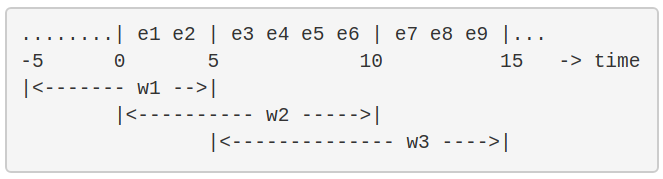
\includegraphics[width=0.7\textwidth]{Figures/SlidingWindow.png}
  \caption{A time duration based sliding window with length 10 secs and sliding interval of 5 seconds.}
  \label{fig:SlideBolt}
\end{figure}

Figure~\ref{fig:SlideBolt} depicts an example of a duration based sliding window with length 10 secs and sliding interval of 5 seconds. The window is evaluated every 10 seconds and some of the tuples in the first window overlaps with the second one. Figure~\ref{fig:WindowBolt} depicts the API to add a rule window with length 10 secs and sliding interval of 5 seconds.

\begin{figure}[h!]
  \centering
  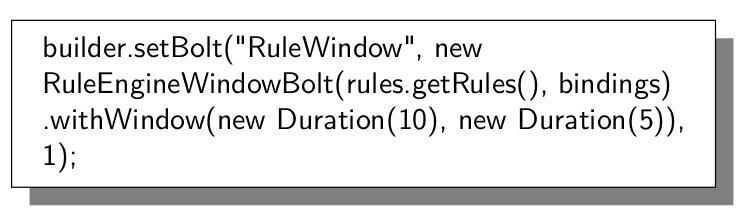
\includegraphics[width=0.7\textwidth]{Figures/WindowBolt.png}
  \caption{Rule engine window bolt definition.}
  \label{fig:WindowBolt}
\end{figure}

Figure~\ref{fig:TumbBolt} depicts a window is evaluated every five seconds and none of the windows overlap.

\begin{figure}[h!]
  \centering
  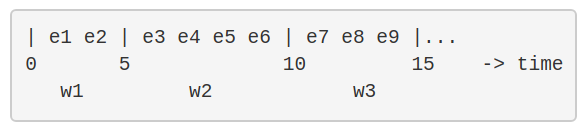
\includegraphics[width=0.7\textwidth]{Figures/TumblingWindow.png}
  \caption{A time duration based tumbling window with length 5 secs..}
  \label{fig:TumbBolt}
\end{figure}


\subsubsection{Data Quality Rule-Based System}

\begin{figure}[h!]
  \centering
  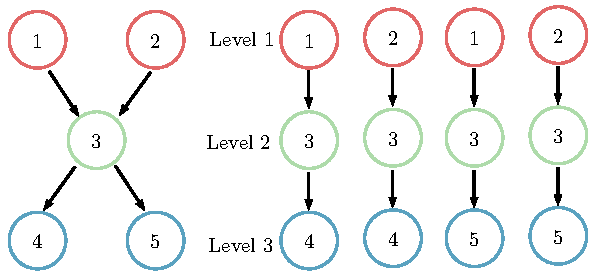
\includegraphics[width=0.6\textwidth]{Figures/AlgoImg.pdf}
  \caption{Storm topology linewise representation}
  \label{fig:AlgoImg}
\end{figure}


The second type of rule are the data quality rules. Our data quality rule-based system (QoS rule-based system) works similarly to the content-driven rule-based system. It consists of a custom Apache Storm stream grouping and a rule engine. In Apache Storm, part of defining a topology is to define how data is exchanged between components (how streams are consumed by the bolts). A Stream Grouping specifies which streams are consumed by each bolt. A stream grouping tells a topology how to send tuples between two components. The rule engine parses the given rule entries and computes all the possible paths that will satisfy the constraints specified by the rules. In order for the stream grouping to determine all the paths that will satisfy the constraints specified by the rules we developed in an offline training mode where the stream grouping collects execution information, transfers information, etc.. to determine all the paths that will satisfy the constraint. The data quality rule entries contain a tag filed and a deadline filed. The tag filed needs to be part of each of the tuples that needs to processed. The deadline filed specifies how much time each tuple with the corresponding tag has to go through the entire Storm topology. The algorithm consists of following steps: (1) breakdown the Storm topology into lines-paths from the task of the first level to the task of the last level through only one child on each level; (2) order lines according to their relative computing times $T_{comp}^l$. (3) iterate over the lines until one of the lines does not meet the deadline $D$ and schedule the work.

\begin{figure}[h!]
  \centering
  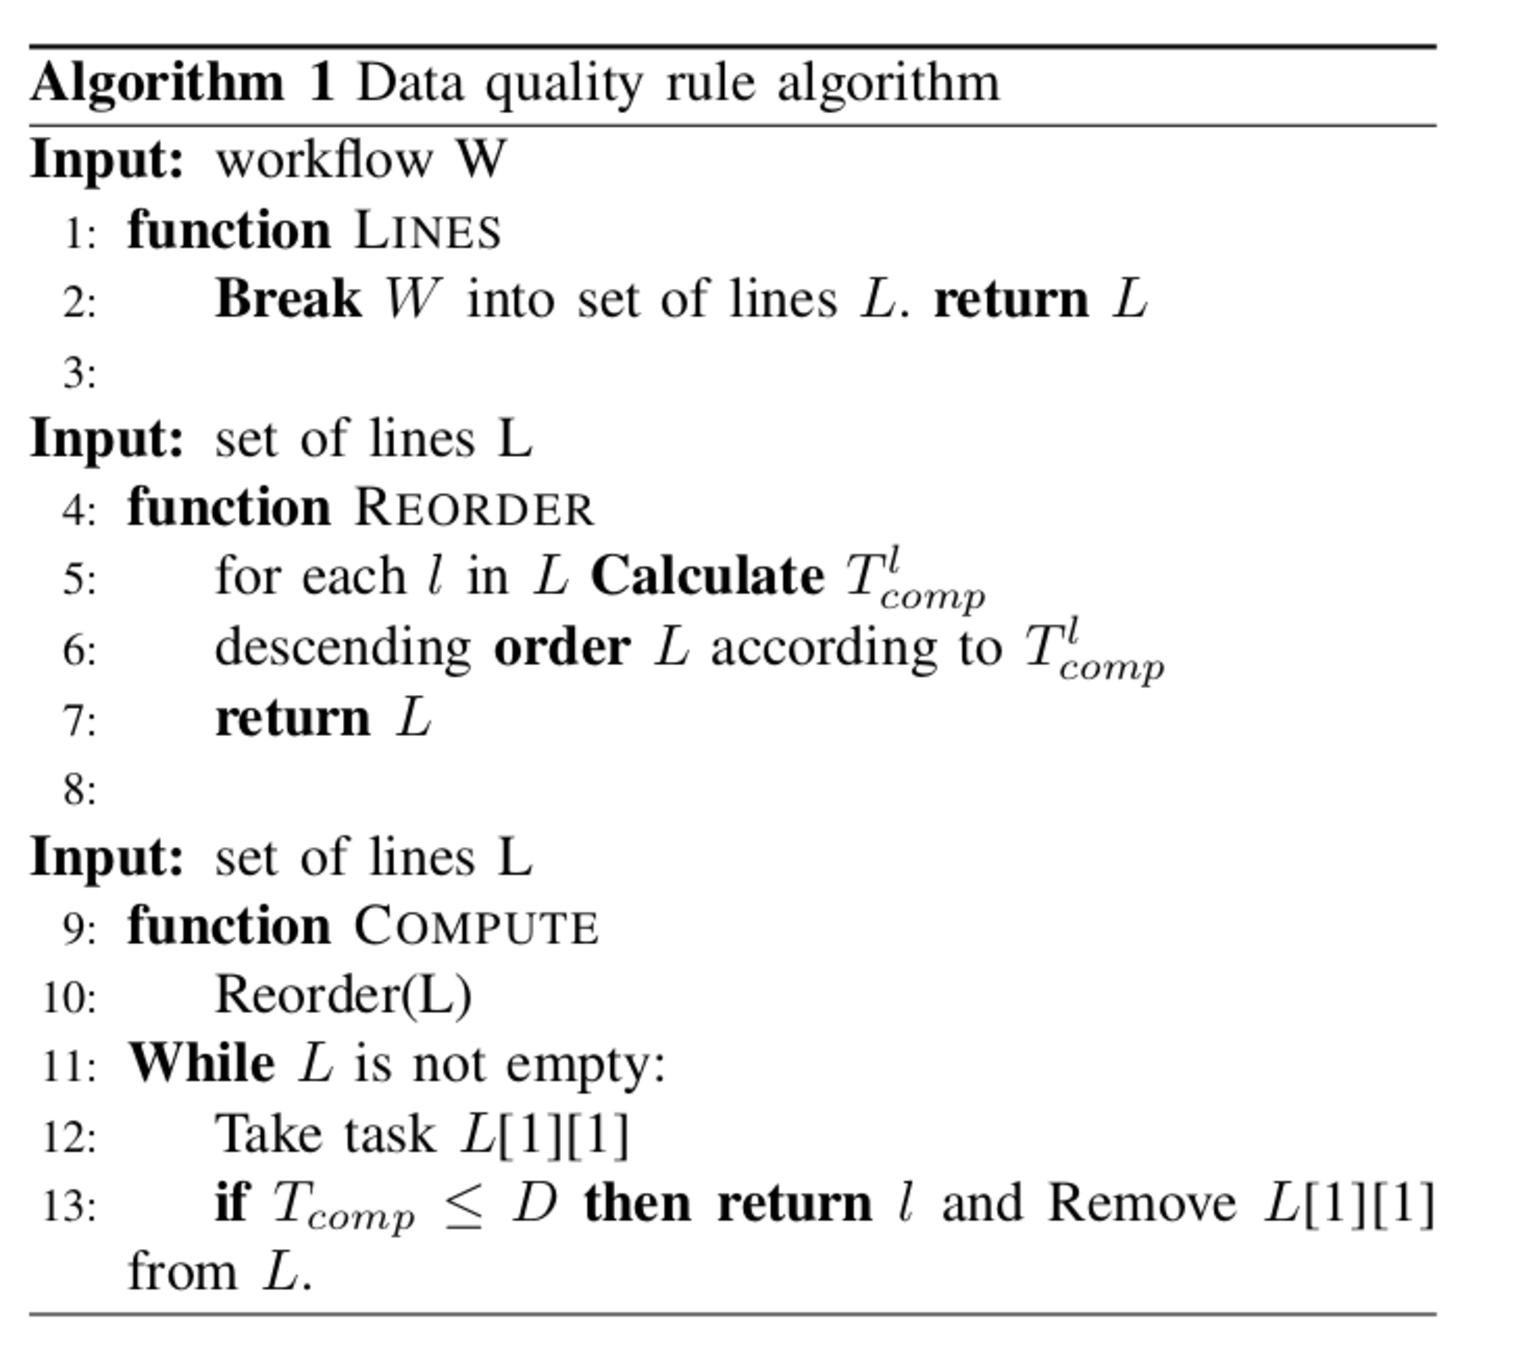
\includegraphics[width=0.7\textwidth]{Figures/Algorithm.pdf}
  \label{fig:Algorithm}
\end{figure}

The overall steps of the algorithm are depicted in Algorithm 1. In the first step of execution process the algorithm creates lines of the topology tasks and calculates the relative computing time $T_{comp}^l$ for each line. $T_{comp}^l$ is calculated as the sum of execution times $T_{comp}^l$ of all tasks in the line. $T_{comp}^l$ consists of task runtime $T_{run}^t$ and total input data transfer time $T_{data}^t$. Then we order all the paths according to their relative computing times $T_{comp}^l$ so we only need to check if $T_{comp}^l$ satisfies the deadline $D$. Once we find one path that does not satisfy the deadline $D$, we have our set of paths that satisfies the constraint and we schedule the work. The algorithm is constantly running and reschedules the work if the computation conditions change.

Figure~\ref{fig:qosRule} presents a brief code example of how developers will express the data quality rules:

\begin{figure}[h!]
  \centering
  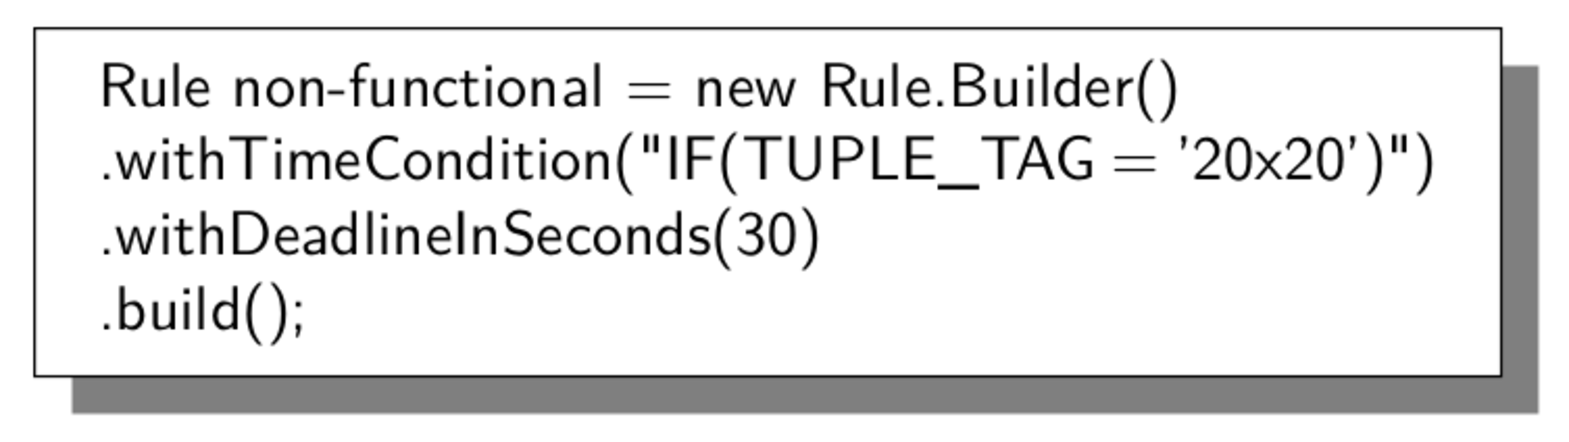
\includegraphics[width=0.7\textwidth]{Figures/qosRule.pdf}
  \caption{}\label{fig:qosRule}
\end{figure}

%\section{Semantics of the Programming Abstraction}
%\section{Realizing Data-Drive Edge Stream Processing}
%\subsection{Basic Functionality}
%\section{Experimental Evaluation}
%\subsection{Scalability and Overhead Experiments}
%\subsection{Performance experiments}
%\section{Summary}